\section{Trigonometrie}

\subsection{Quadrantenbeziehungen}
\begin{tabbing}
	xxxxxxxxxxxxxxxxxxxxxxxxxxxxxxxxxx \= \kill
	$\sin(-a)=-\sin(a)$ \> $\cos(-a)=\cos(a)$\\
	$\sin(\pi - a)=\sin(a)$ \> $\cos(\pi - a)=-\cos(a)$\\
	$\sin(\pi + a)=-\sin(a)$ \> $\cos(\pi +a)=-\cos(a)$\\
	$\sin\left(\frac{\pi}{2}-a \right)=\sin\left(\frac{\pi}{2}+a \right)=\cos(a)$ \>
	$\cos\left(\frac{\pi}{2}-a \right)=-\cos\left(\frac{\pi}{2}+a \right)=\sin(a)$  
\end{tabbing}

\subsection{Ableitungen}

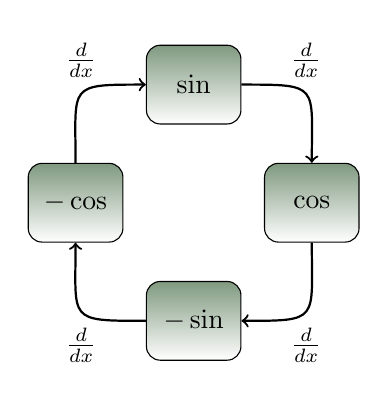
\begin{tikzpicture}
	[	inner sep = 2mm,
	sin/.style={rectangle,minimum width=1.2cm,minimum height=1cm,rounded corners=5pt,draw=black,top color=green!20!black!50},
	abl/.style={rectangle}
	]
	\node at (1.5,0) (sin1) [sin] {$\sin$};
	\node at (0,-1.5) (cos2) [sin] {$-\cos$};
	\node at (1.5,-3) (sin2) [sin] {$-\sin$};
	\node at (3,-1.5) (cos1) [sin] {$\cos$};
	
	\draw[thick,black,->] (sin1.east) .. controls +(right:1cm) and +(up:1cm) ..  (cos1.north)
	node [pos=0.5,above](abl) {$\frac{d}{dx}$};
	\draw[thick,black,->] (cos1.south) .. controls +(down:1cm) and +(right:1cm) .. (sin2.east)
	node [pos=0.5,below](abl) {$\frac{d}{dx}$};
	\draw[thick,black,->] (sin2.west) .. controls +(left:1cm) and +(down:1cm) .. (cos2.south)
	node [pos=0.5,below](abl) {$\frac{d}{dx}$};
	\draw[thick,black,->] (cos2.north) .. controls +(up:1cm) and +(left:1cm) .. (sin1.west)
	node [pos=0.5,above](abl) {$\frac{d}{dx}$};
\end{tikzpicture}

\begin{minipage}{0.5\textwidth}
\subsection{Additionstheoreme}
	$\sin(a \pm b)=\sin(a) \cdot \cos(b) \pm \cos(a) \cdot \sin(b)$\\
	$\cos(a \pm b)=\cos(a) \cdot \cos(b) \mp \sin(a) \cdot \sin(b)$\\	
	$\tan(a \pm b)=\dfrac{\tan(a) \pm \tan(b)}{1 \mp \tan(a) \cdot \tan(b)}$
\end{minipage}
%
\begin{minipage}{0.5\textwidth}
\subsection{Doppel- und Halbwinkel}	
	$\sin(2a)=2\sin(a)\cos(a)$\\
	$\cos(2a)=\cos^2(a)-\sin^2(a)=2\cos^2(a)-1=1-2\sin^2(a)$\\
	$\cos^2 \left(\frac{a}{2}\right)=\frac{1+\cos(a)}{2} \qquad
	\sin^2 \left(\dfrac{a}{2}\right)=\frac{1-\cos(a)}{2}$
\end{minipage}
%

\subsection{Euler-Formeln} 
	$\sin(x) = \frac{1}{2j} \left(e^{jx} - e^{-jx}\right)$ \\
	$\cos(x) = \frac{1}{2} \left(e^{jx} + e^{-jx}\right)$ \\
	$e^{x+jy} = e^x \cdot e^{jy} = e^x \cdot \left(\cos(y) + j\sin(y)\right)$ \\
	$e^{j\pi} = e^{-j\pi} = -1$ \\

\subsection{Periodizität}
	$\cos(a+k\cdot2\pi)=\cos(a) \qquad \sin(a+k\cdot2\pi)=\sin(a) \qquad
	(k \in \mathbb{Z})$

\subsection{Produkte}
	$\sin(a)\sin(b)=\frac{1}{2}(\cos(a-b)-\cos(a+b))$\\
	$\cos(a)\cos(b)=\frac{1}{2}(\cos(a-b)+\cos(a+b))$\\
	$\sin(a)\cos(b)=\frac{1}{2}(\sin(a-b)+\sin(a+b))$\\

\subsection{Summe und Differenz}
	$\sin(a)+\sin(b)=2 \cdot \sin \left(\frac{a+b}{2}\right) \cdot
	\cos\left(\frac{a-b}{2}\right)$\\
	$\sin(a)-\sin(b)=2 \cdot \sin \left(\frac{a-b}{2}\right) \cdot
	\cos\left(\frac{a+b}{2}\right)$\\
	$\cos(a)+\cos(b)=2 \cdot \cos \left(\frac{a+b}{2}\right) \cdot
	\cos\left(\frac{a-b}{2}\right)$\\
	$\cos(a)-\cos(b)=-2 \cdot \sin \left(\frac{a+b}{2}\right) \cdot
	\sin\left(\frac{a-b}{2}\right)$\\
	$\tan(a) \pm \tan(b)=\dfrac{\sin(a \pm b)}{\cos(a)\cos(b)}$\\

\subsection{Funktionswerte für Winkelargumente}
\begin{multicols}{4}	
	\begin{tabular}[c]{|p{0.5cm}|p{0.4cm}||p{0.4cm}|p{0.4cm}|p{0.4cm}|}
		\hline
		deg & rad & sin & cos & tan\\
		\hline
		0\symbol{23} & 0 & 0 & 1 & 0\\
		\hline
		30\symbol{23} & $\frac{\pi}{6}$ & $\frac{1}{2}$ & $\frac{\sqrt{3}}{2}$ &
		$\frac{\sqrt{3}}{3}$\\
		\hline
		45\symbol{23} & $\frac{\pi}{4}$ & $\frac{\sqrt{2}}{2}$ & $\frac{\sqrt{2}}{2}$
		& 1\\
		\hline
		60\symbol{23} & $\frac{\pi}{3}$ & $\frac{\sqrt{3}}{2}$ & $\frac{1}{2}$ &
		$\sqrt{3}$\\
		\hline			
	\end{tabular} \\
	
	\begin{tabular}[c]{|p{0.6cm}|p{0.6cm}||p{0.6cm}|p{0.6cm}|}
		\hline
		deg & rad & sin & cos\\
		\hline
		90\symbol{23} & $\frac{\pi}{2}$ & 1 & 0\\
		\hline	
		120\symbol{23} & $\frac{2\pi}{3}$ & $\frac{\sqrt{3}}{2}$ & $-\frac{1}{2}$ \\
		\hline
		135\symbol{23} & $\frac{3\pi}{4}$ & $\frac{\sqrt{2}}{2}$ & $-\frac{\sqrt{2}}{2}$\\
		\hline
		150\symbol{23} & $\frac{5\pi}{6}$ & $\frac{1}{2}$ & $-\frac{\sqrt{3}}{2}$\\
		\hline
	\end{tabular} \\
	
	\begin{tabular}[c]{|p{0.6cm}|p{0.6cm}||p{0.6cm}|p{0.6cm}|}
		\hline
		deg & rad & sin & cos\\
		\hline
		180\symbol{23} & $\pi$ & 0 & -1\\
		\hline	
		210\symbol{23} & $\frac{7\pi}{6}$ & $-\frac{1}{2}$ & $-\frac{\sqrt{3}}{2}$\\
		\hline
		225\symbol{23} & $\frac{5\pi}{4}$ & $-\frac{\sqrt{2}}{2}$ & $-\frac{\sqrt{2}}{2}$\\
		\hline
		240\symbol{23} & $\frac{4\pi}{3}$ & $-\frac{\sqrt{3}}{2}$ & $-\frac{1}{2}$\\
		\hline
	\end{tabular} \\
	
	\begin{tabular}[c]{|p{0.6cm}|p{0.6cm}||p{0.6cm}|p{0.6cm}|}
		\hline
		deg & rad & sin & cos\\
		\hline
		270\symbol{23} & $\frac{3\pi}{2}$ & -1 & 0\\
		\hline	
		300\symbol{23} & $\frac{5\pi}{3}$ & $-\frac{\sqrt{3}}{2}$ & $\frac{1}{2}$\\
		\hline
		315\symbol{23} & $\frac{7\pi}{4}$ & $-\frac{\sqrt{2}}{2}$ & $\frac{\sqrt{2}}{2}$\\
		\hline
		330\symbol{23} & $\frac{11\pi}{6}$ & $-\frac{1}{2}$ & $\frac{\sqrt{3}}{2}$\\
		\hline
	\end{tabular}					
\end{multicols}